% !TeX spellcheck = pt_PT
\documentclass[a4paper]{report}
\usepackage[portuguese]{babel}
\usepackage{a4wide}

\usepackage{graphicx}
\usepackage{hyperref}
\usepackage{listings}
\usepackage{indentfirst}
\usepackage{float}

\setlength{\parskip}{1em}

\title{POO-Sistema de Gestão de Encomendas\\
	\large Grupo 33}
\author{Sofia Santos (A89615)
	\and Ana Filipa Pereira (A89589)
	\and Carolina Santejo (A89500)}
\date{Ano Letivo 2019/2020}

\begin{document}
	\begin{minipage}{0.9\linewidth}
        \centering
		
\includegraphics[width=0.4\textwidth]{eng.jpeg}\par\vspace{1cm}
		\href{https://www.uminho.pt/PT}
		{\scshape\LARGE Universidade do Minho} \par
		\vspace{0.6cm}
		\href{https://miei.di.uminho.pt/}
		{\scshape\Large Mestrado Integrado em Engenharia Informática} \par
		\maketitle
		\begin{figure}[H]
			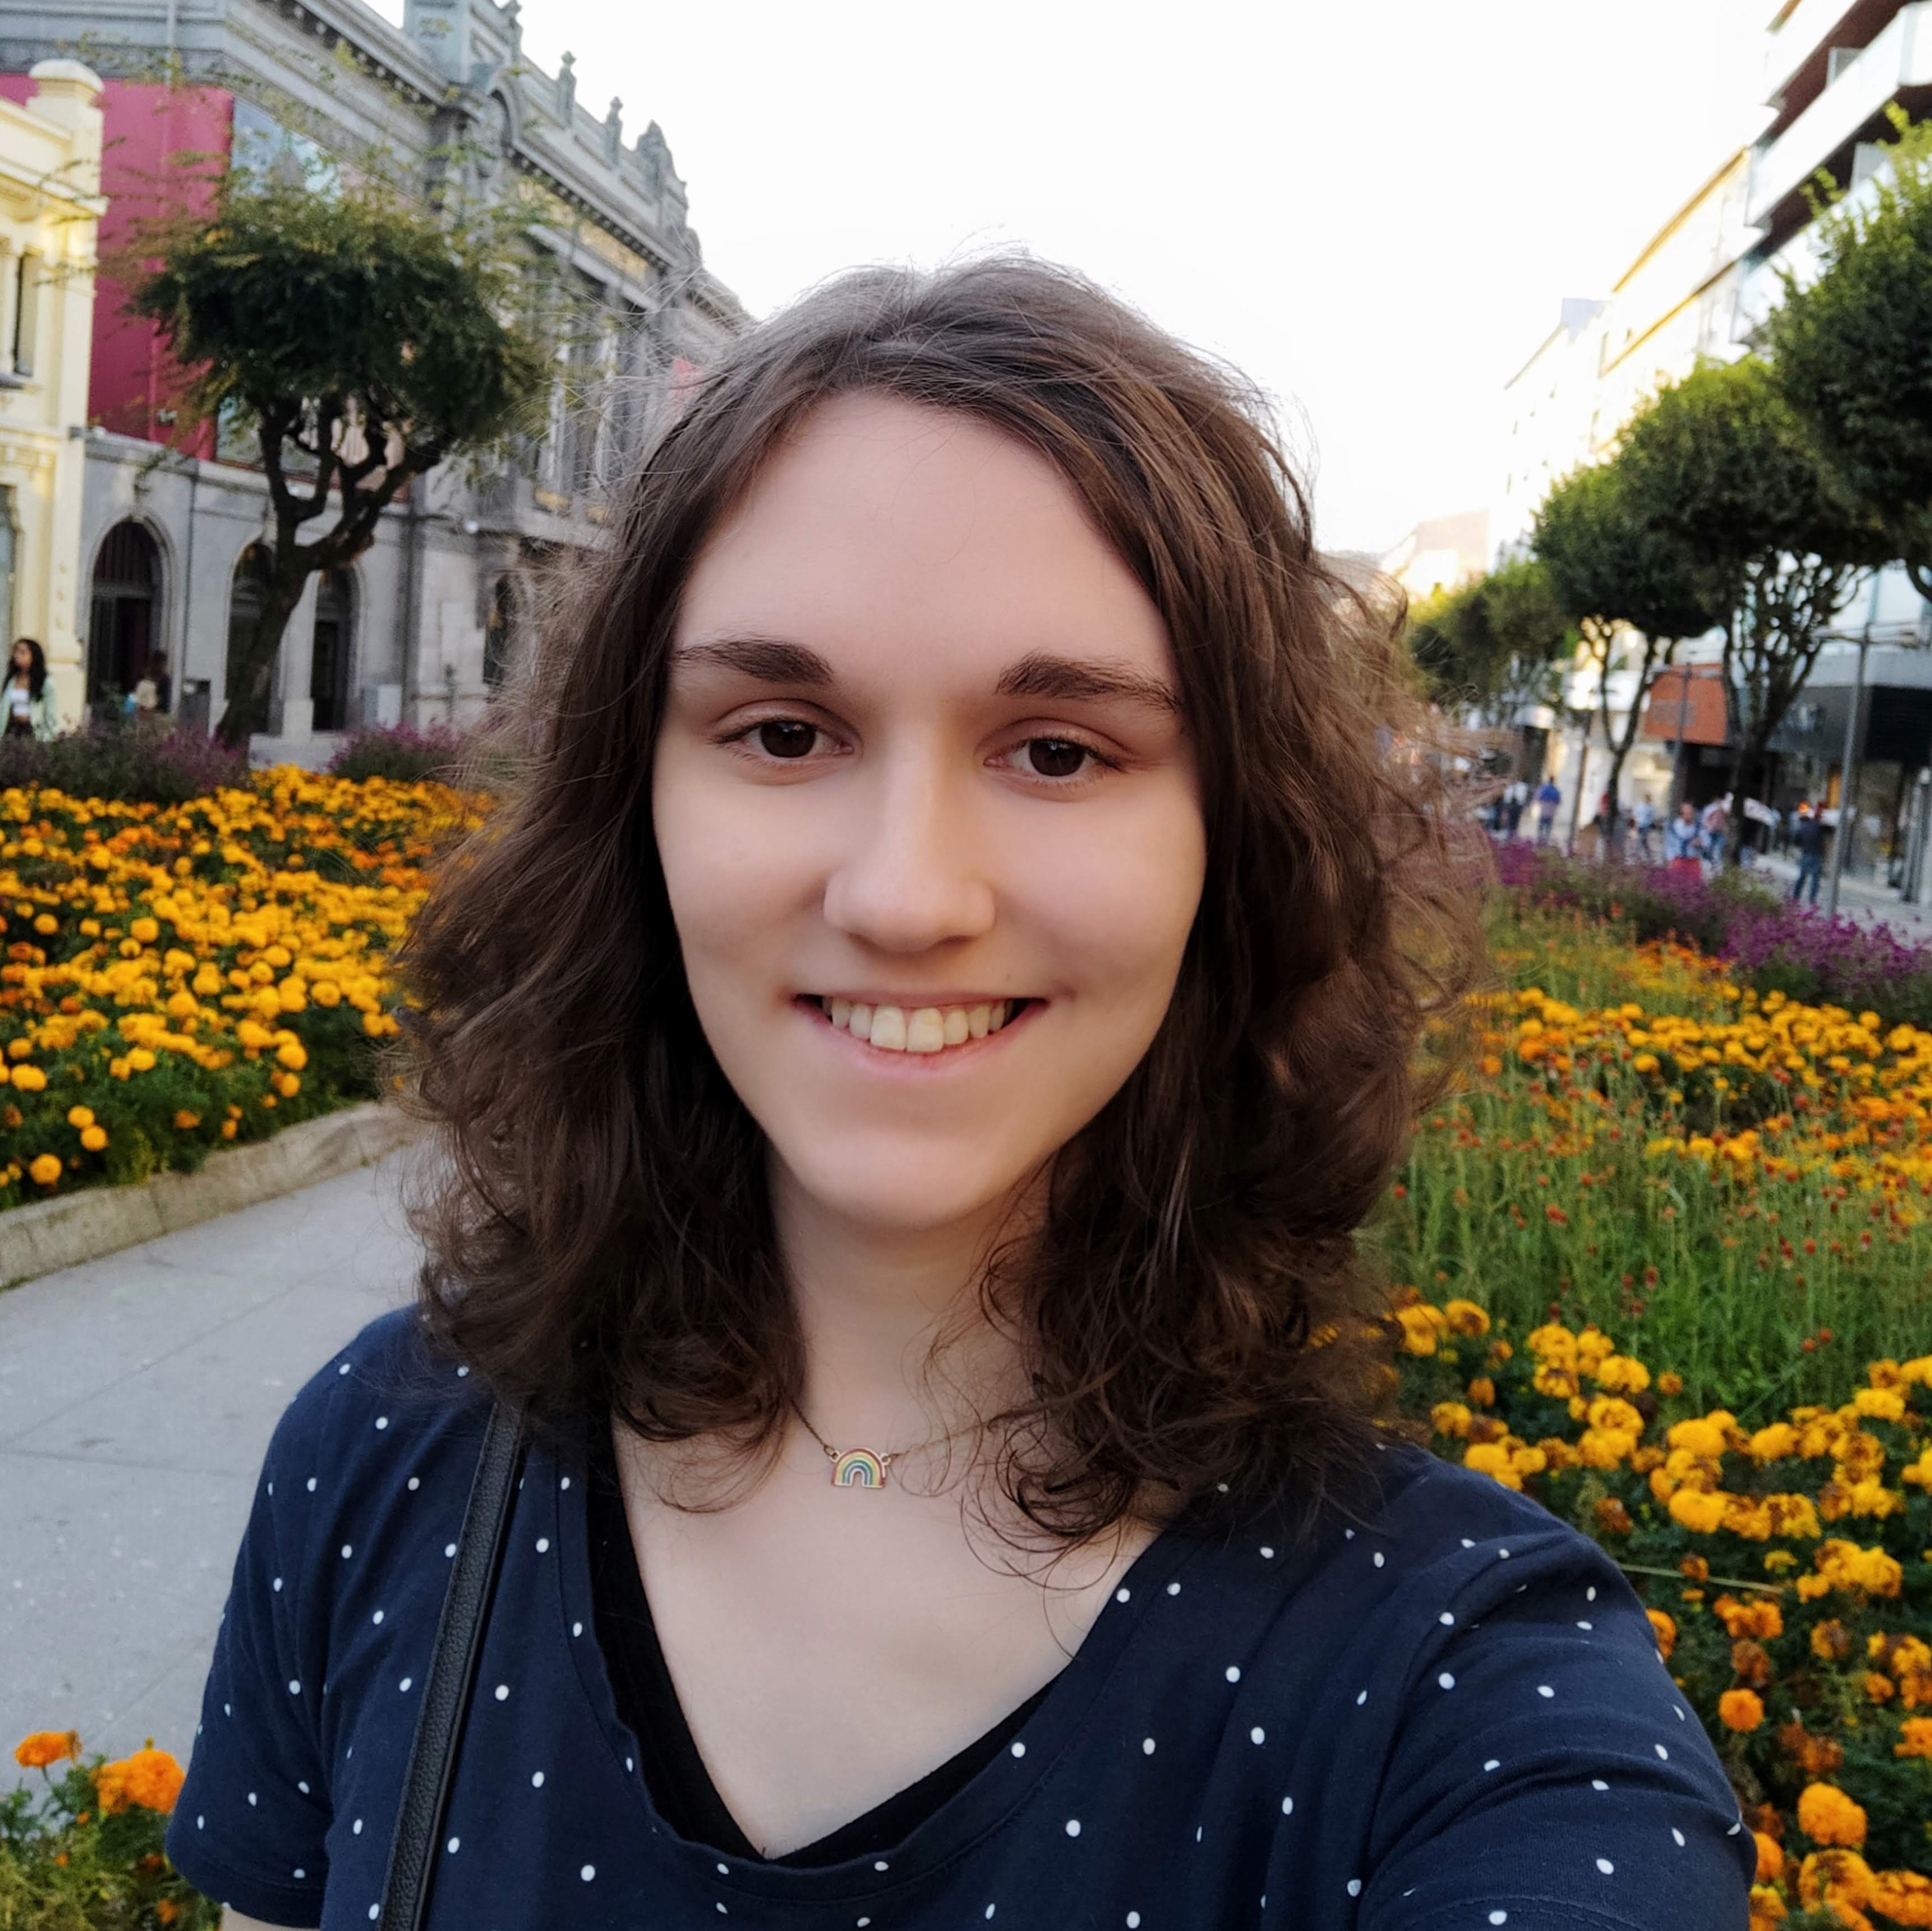
\includegraphics[width=0.32\linewidth]{sofia.jpg}
			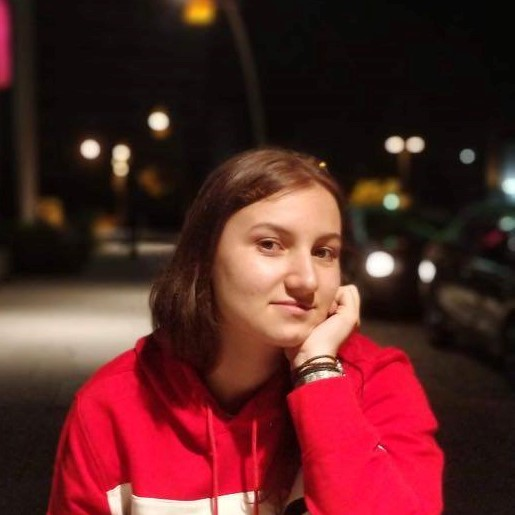
\includegraphics[width=0.32\linewidth]{filipa.jpg}
			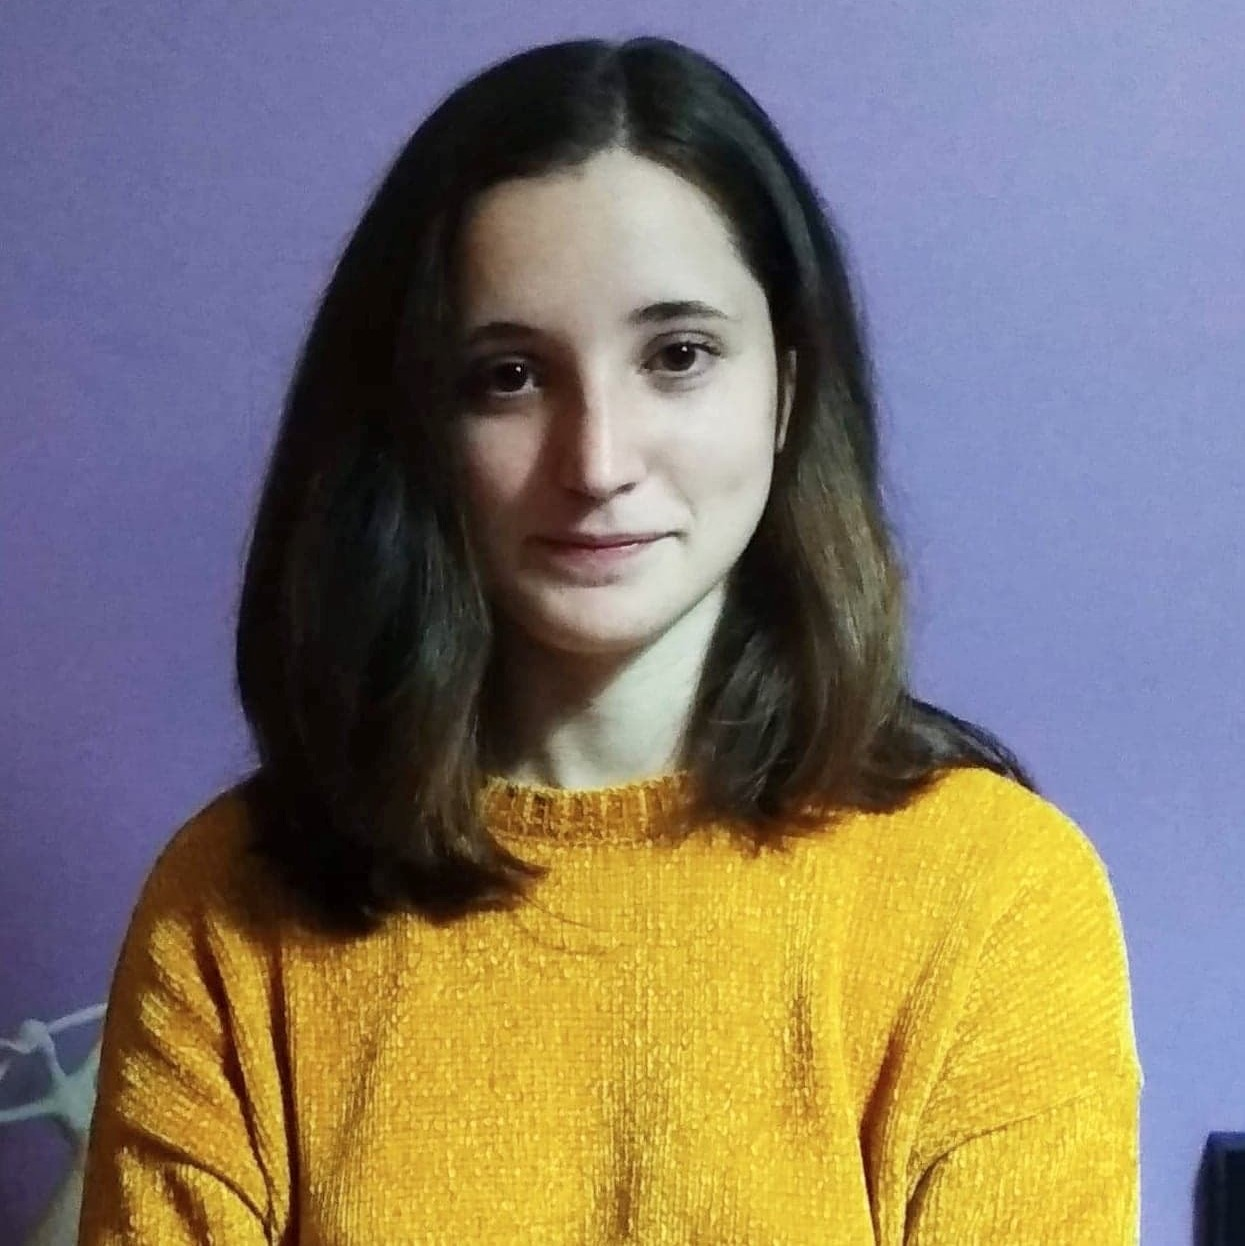
\includegraphics[width=0.32\linewidth]{santejo.jpg}
		\end{figure}
	\end{minipage}
	
	\tableofcontents
	
	\pagebreak
	
	\chapter{Introdução e principais desafios}
%	
	Este projeto consistiu no desenvolvimento de um Sistema de Gestão de Encomendas na linguagem de programação Java,de forma a pôr em prática os conhecimentos adquiridos ao longo so semestre. 
	
	Consideramos que o maior desafio tenha sido gerir várias encomendas, de diferentes naturezas, e várias entidades em simultâneo, tendo em conta fatores aleatórios, tais como atrasos nas filas de espera das lojas, ou atrasos nos deslocamentos das entidades Voluntarios e Transportadoras.
	
	\chapter{Classes}
	\section{Main}
	Classe responsável por arrancar com o programa.Para isto o método \textit{main} chama o método \textit{main} da classe \textit{controler};
	
	\section{TrazAqui}
	\begin{lstlisting}[language=Java]
	private Conta contaLoggedIn;
	private Estado estado;
	\end{lstlisting}
	TrazAqui é uma das várias classes controladoras do sistema;
	A classe TrazAqui é a classe que associa a conta com que se fez login a todo o estado atual do programa.Decidimos que a relação entre esta classe e Estado seria de agregação, pois ao partilhar o apontador da conta, caso esta seja alterada no Estado, o atributo contaLoggedIn será automaticamente alterado.
	\section{Estado}
	\begin{lstlisting}[language=Java]
	private Contas utilizadores;
	private Contas voluntarios;
	private Contas transportadoras;
	private Contas lojas;
	private Encomendas encomendas;
	private Set<AbstractMap.SimpleEntry<String, String>> pedidosTransporte; // -> (codEnc, Codt)
	\end{lstlisting}
	
	Estado é uma das várias classes controladoras do sistema.
	A classe Estado é a classe responsável por gerir toda a informação do sistema.Como podemos ver, esta possui a informação de todas as contas registadas no sistema e todas as encomendas registadas na aplicação.O atributo pedidosDeTransporte consiste num Set em que cada elemento é um "par" constituido pelo código da Transportadora e pelo código da Encomenda que aquela deseja transportar. Este pedido é retirado do Set se o pedido for aprovado ou outra entidade tenha ficado responsável pelo transporte da encomenda.A uníca relacão de agregação entre classes em todo o programa é entre o Estado e a TrazAqui(falaremos disso novamente).
	
	\section{Controller}
	Classe, que juntamente com outras, gere o fluxo da aplicação.Esta é a classe responsável por gerir o menu inicial, disponível para todas as entidades,além de interagir com outras classes controladoras que gerem os menus de cada entidade em particular (\textit{login});
	O método run de cada controller das entidades recebe um objecto de TrazAqui, de forma a que tenham acesso á informação que necessitam que se encontra ,por exemplo,no estado.


    \section{ControllerUtilizador}
    Umas das várias classes controladoras do sistema. Esta em particular é a que gere o menu do utilizador; 
    
      Neste menu temos as seguintes opções:
      
      \textit{1-Efetuar uma compra}: Esta será adicionada á fila de espera da Loja.
      
      \textit{2-Solicitar Encomeda}: Só após selecionar esta opção e escolher a encomenda que quer solicitar,é que essa encomenda estará disponível para ser escolhida pelas entidades de transporte.
      
      \textit{3-Verificar ofertas da Transportadora}: Caso alguma transportadora tenha desejado transportar uma das encomendas do  utilizador, este terá acesso ao código da transportadora, ao tempo que (em teoria) demorará o transporte e ao custo(que poderá variar dependendo da rota do transportador). Com isto o utilizador pode aceitar ou recusar o pedido.
      
      \textit{4-Historico}: Devolve o histórico das encomendas transportadas entre duas datas.
      
      \textit{5-Classificar Entidade}: Permite que o utilizador classifique uma entidade, mas com a condição de que esta tenha que já transportado para o dito utilizador. 
      
      \textit{6-Numero de encomendas Transportadas}:Devolve o número de encomendas transportadas ao utilizador.
    
	\section{ControllerVoluntario}
	   Umas das várias classes controladoras do sistema. Esta em particular é a que gere o menu do voluntário;
	   
	   Neste menu temos as seguintes opções:
	   
	   \textit{1-Selecionar encomenda para transportar}: Caso o voluntário esteja disponivel(ou sej, não tenha mais nenhuma encomenda na sua posse), aparecerão todas as encomendas solicitadas e dentro dos seus limites de escolha(ex. raio). Este pode aceitar ou não.
	   
	   \textit{2-Fazer Entrega}:O voluntário encrementa o número de encomendas transportadas do utilizador,é mostrado o tempo que efetivamente demorou, contando com atrasos e filas de espera.
	   
	   \textit{3-Verificar classificacao}: Devolve a média de todas as classificações atribuidas.
	   
	   \textit{4-Historico}: Devolve o histórico das encomendas transportadas entre duas datas.
	   

	\section{ControllerLoja}
	 Umas das várias classes controladoras do sistema. Esta em particular é a que gere o menu da Loja;
	 
	 Neste menu temos as seguintes opções:
	 
	 \textit{1-Ver lista de encomenda}: Mostra todas as encomendas na fila de espera.
	 \textit{1-Despachar Encomenda }: Encomenda deixa de estar na fila de espera e passa para a lista de encomendas despachadas;
	 
	 \textit{2-Quanto falta até encomenda estar disponível}:Caso a encomenda se encontre na loja, devolve o tempo teórico que demorará até ficar despachada(relembrando que poderá haver atrasos oua encomenda se despachar mais rápido);
	
	\section{ControllerTransportadora}
	 Umas das várias classes controladoras do sistema. Esta em particular é a que gere o menu da Transportadora;
	 
	 Neste menu temos as seguintes opções:
	 
	 \textit{1-Preço de transporte de uma encomenda}: Caso a transportadora possa transportar a encomenda, é devolvido o preço do transporte, tendo em conta a distância e o peso da mesma.
	 
	  \textit{2-Fazer Entrega}:A transportadora define uma rota e vai distribuindo as encomendas guardando as distâcias parciais percorridas.(Ela primeiro vai a todas as lojas e depois a todos os utilizadores.)
	  
	  \textit{3-Total faturado num período}:Dado que as encomendas guardam quem as transportou, a distância para a ir buscar e entregar e a data, foi apenas necessário buscar as encomendas que satisfazem os requesitos e somar o custo de cada uma.
	 
	 \textit{4-Selecionar encomenda para transportar}: Caso a transportadora esteja disponivel(ou seja,o numero de encomendas é inferior ao máximo suportado), aparecerão todas as encomendas solicitadas e dentro dos seus limites de escolha(ex. raio). Este pode aceitar ou não.Caso aceite tem de aguardar aprovação do utilizador.
	 
	\textit{5-Verificar classificacao}: Devolve a média de todas as classificações atribuidas.
	 
	 \textit{6-Historico}: Devolve o histórico das encomendas transportadas entre duas datas.
	
	\section{Conta}
	\begin{lstlisting}[language=Java]
	private String codigo;
	private String nome;
	private Point2D gps;
	private String email;
	private String password;
	\end{lstlisting}
	Esta classe faz parte do Modelo da aplicação. Conta é superclasse de todas as outras classes que representam as entidades do sistema. Os seus atributos são aqueles comuns a essas mesmas entidades.
	
	\section{Contas}
	\begin{lstlisting}[language=Java]
	private Map<String,Conta> mapContas;
	\end{lstlisting}
	Esta classe faz parte do Modelo da aplicação. A classe Contas é responsável por armazenar todas as contas do Sistema. Para tal escolhemos uma estrutura Map, na qual ada conta fica associada ao seu código;
	
	
	
	\section{Encomenda}
	\begin{lstlisting}[language=Java]
	private String codEnc;
	private String codUtil;
	private String codLoja;
	private double peso;
	private Map<String, LinhaEncomenda> produtos;
	private LocalDateTime data;
	private boolean foiSolicitada;
	private boolean foiEntregue;
	private String quemTransportou;
	private boolean encMedica;
	private double distPercorrida;
};
   
	\end{lstlisting}
	A classe Encomenda possui todos os atributos mínimos exigidos pelos docentes, no entanto tomámos a liberdade de adicionar 4 novos atributos:
	
	  	\textit{LocalDateTime data} - data do Transporte da encomenda
	  	
	  \textit{boolean foiSolicitada} -Indica se a encomenda foi solicitada pelo utilizador
	  
	  \textit{boolean foiEntregue}  - Indica se a encomenda chegou a ser entregue 
	  
	  \textit{String quemTransportou} - código de quem a transportou;
	  
	  \textit{boolean encMedica} - Indica se a encomenda é médica ou não
	  
	  \textit{distPercorrida} - distância percorrida pela entidade de transporote para entregar  	essa encomenda;
	  
	
		\section{LinhaEncomenda}
	\begin{lstlisting}[language=Java]
	private String codProduto;
	private String descricao;
	private double quantidade;
	private double valorUnitario;
	};
	
	\end{lstlisting}
		Os atributos desta classe são em tudo semelhante aos atributos mínimos exigidos.
		
	\section{Utilizador}
	Uma das subclasses da classe Conta, e que faz parte do Modelo do Sistema.	
	
	Cada utilizador,além de possuir os atributos da classe conta, possui também o atributo:
	\begin{lstlisting}[language=Java]
	private int encTransportadas;
	\end{lstlisting}
	que indica quantas encomendas foram transportadas para o utilizador(cada vez que um voluntário ou transportadora efetua o transporte um método incrementa o valor de encTransportadas);
	
	
	\section{Voluntario}
	Uma das subclasses da classe Conta, e que faz parte do Modelo do Sistema;
	
	Cada voluntario,além de possuir os atributos da classe conta, possui também os atributos:
	\begin{lstlisting}[language=Java]
	private double raio;
	private String encAceite; //Encomenda que aceitou
	private boolean disponivel;
	private List<Integer> classificacao;
	private boolean medicamentos;
	private double velocidade; 
	\end{lstlisting}
	Destas, aquelas que foram acrescentadas por decisão do grupo foram as seguintes:
 	
\textit{String encAceite} -Indica qual a encomenda na posse do voluntário para entregar

\textit{boolean disponivel}  - Indica se o voluntário pode receber uam nova encomenda(se já tiver aceitado uma encomenda, então não está disponível)

\textit{List<Integer> classificacao} - Todas as classificações atribuidas ao voluntário.

\textit{boolean medicamentos} - Indica se o voluntario pode transportar encomendas médicas

\textit{double velocidade} - velocidade média a que o voluntário de desloca;
	
	\section{Loja}
	Uma das subclasses da classe Conta, e que faz parte do Modelo do Sistema;
	
	Cada loja,além de possuir os atributos da classe conta, possui também os atributos:
	\begin{lstlisting}[language=Java]
	private Queue<Encomenda> filaEspera;
	private double tempoEsperaIndividual;
	private List<Encomenda> encProntas;
	\end{lstlisting}
	\textit{Queue<Encomenda> filaEspera} - fila com os códigos de encomendas á espera para serem despachados; 
	
	\textit{ List<Encomenda> encProntas} - fila com todas as encomendas despachadas pela loja. Não há tempo de espera neste caso.
	
	\textit{ double tempoEsperaIndividual} - tempo médio de espera, por pessoa, na fila da loja, sendo que este tempo pode ser superior caso haja atrasos. Falaremos disso daqui a pouco.
	
	
	\section{Transportadora}
	Uma das subclasses da classe Conta, e que faz parte do Modelo do Sistema;
	
	Cada transportadora,além de possuir os atributos da classe conta, possui também os atributos:
	\begin{lstlisting}[language=Java]
	private String nif;
	private double raio;
	private double precoKm;
	private double precoKg;
	private List<Integer> classificacao;
	\end{lstlisting}
	\textit{List<Integer> classificacao} - Todas as classificações atribuidas á transportadora.
	
	\section{Menu}
	O Menu é a Vista do programa. Comunica apenas com o Controller e os Controllers das entidades.
	Possui vários métodos,nomeadamente para receber algum tipo de informação da entidade que usa a app, para mostrar algum tipo de informação ou mostrar mensagens de erro.
	
	\section{Interface Randoms}
	De forma a tentar resolver o problema da gestão de tempos de fila de espera e os atrasos no deslocamento das entidades de transporte, criamos a inteface Random, apenas com métodos default, que se baseiam essencialmente em probabilidades.
	De forma resumida acontece o seguinte:
	 - Quando entidade de transporte chega á loja pra pegar a encomenda, a sua entrega pode ser despachada mais rápido, logo o tempo na fila de espera será menor do que o inicialmente pensado, ou a sua entrega pode ser atrasada e assim o tempo na fila de espera será maior.
	 
	 - Quando entidade de transporte está a realizar a entrega existe a probabilidade de haver um atraso. Caso isto se verifique, implementamos ainda a ideia de que há 3 tipos de atraso: um pequeno atraso, um atraso médio, ou um grande atraso.
	 
	 Em ambos os casos os tempos são gerados aleatoriamente. 
	 
	  \section{Interface TranspVolunt}
	 Inteface com métodos comuns a ambos os voluntários e transportadoras.
	 
	 \section{TipoConta}
	 A classe Enum TipoConta permite que os vários tipos decontas sejam encarados como "constantes" e foi-nos útil para situações que dependendo da conta uma condição diferente teria de ser realizada. Por exemplo, ao fazer login, será devolvido um TipoConta, sendo que dependendo deste será invocado o método run em uma das classes controladoras das entidades.
	 
	\section{Point}
	Classe com métodos que transforma as latitudes e longitudes em distâncias em KM.
	\chapter{Estrutura do projeto}
	
	O nosso projeto segue a estrutura \textit{Model View Controller} (MVC), estando por isso organizado em três camadas:
	\begin{itemize}
		\item A camada de dados (o modelo) é composta pelas Classes da Entidades e pelas classes Main, Conta,Contas, Encomendas,Encomenda,LinhaEncomendae e pelas interfaces.
		\item A camada de interação com o utilizador (a vista, ou apresentação) é composta unicamente pela classe Menu.
		\item A camada de controlo do fluxo do programa (o controlador) é composta pela classe Controller, pelo Controller das Entidades,e pelas classes Estado e TrazAqui, sendo que destas apenas a Controller e Controller das Entidades acede á vista diretamente.
	\end{itemize}
      Como foi referido anteriormente, todo o projeto baseia-se na ideia de encapsulamento, á exceção das classes Estado e TrazAqui cuja relação é de agregação. Escolhemos est relação para estas duas classes especificamente pelo simples motivo de que ao partilhar,o apontador da conta com que se fez login, se este for mudado no Estado , a contaLoggedIn em TrazAqui é mudada automaticamnte, algo que seria mais trabalhoso caso a relação fosse de composição.
      

	
	

	\chapter{Conclusão}

	A nível geral, e tendo em conta o que foi explicado nos capítulos anteriores, podemos afirmar que temos um projeto bem conseguido. Pensamos que respondémos de forma correta ao problema da gestão de factores de aleatoriedade,que era a principal dificuldade do trabalho, além de termos implementado as regras de encapsulamento(tirando a exceção já referida) e a possibilidade do nosso projeto crescer de forma controlada.
	
	\appendix
	
	\chapter{Diagrama de Classes}
	
\end{document}